\documentclass[12pt]{article}

\usepackage{amsmath}
\usepackage{amssymb}
\usepackage{graphicx}
\usepackage{float} % for [H] exact placement of floats

% --- ADDED: table styling packages & colors ---
\usepackage{booktabs}
\usepackage[table]{xcolor}
\usepackage{tabularx}  % auto-stretch columns to width
\usepackage{array}
\usepackage{listings} % For code snippets
% Listings configuration for code blocks
\lstset{
    language=C++,
    basicstyle=\ttfamily\small,
    frame=single,
    captionpos=b,
    breaklines=true,
    breakatwhitespace=true,
    numbers=left,
    numberstyle=\tiny\color{gray},
    xleftmargin=1em,
    tabsize=2,
    mathescape=false
}



\definecolor{tbl-hdr}{HTML}{0F172A}   % header background
\definecolor{tbl-rowA}{HTML}{0B1020}  % zebra A
\definecolor{tbl-rowB}{HTML}{141B2C}  % zebra B
\definecolor{tbl-accent}{HTML}{4CC3FF}% header underline
\definecolor{tbl-text}{HTML}{DCE7FF}  % light text
\newcolumntype{L}[1]{>{\raggedright\arraybackslash}p{#1}}
\newcolumntype{C}[1]{>{\centering\arraybackslash}p{#1}}
% --- END ADDED ---

\usepackage{hyperref}
\usepackage{algorithm}
\usepackage{algorithmicx}
\usepackage{algpseudocode}
\usepackage{fancyhdr}
\usepackage{pdflscape}
\usepackage{pdfpages}

\title{CIS 5800 Machine Perception Homework-2 \\ University of Pennsylvania}
\author{Navjot Singh Chahal \\ \href{mailto:nschahal@seas.upenn.edu}{nschahal@seas.upenn.edu}}
\date{\today}

\pagestyle{fancy}
\fancyhf{}
\fancyhead[C]{CIS 5800 Machine Perception HW2 University of Pennsylvania}
\fancyfoot[R]{\thepage}
\fancyfoot[L]{Navjot Singh Chahal}

\begin{document}

\maketitle

\section*{1.1}
The cross-ratio of four collinear points is invariant under a perspective projection.
This means cross-ratio of the points in the 3D world is the same as the cross-ratio of their corresponding points in the 2D image.
\\
\textbf{Note!} Given that in the world, the points are equally spaced, so choosing a 1D parameterization along the line for simplicity.

\[
A_W=0,\quad B_W=1,\quad C_W=2,\quad D_W=3 .
\]
The cross ratio is invariant under projection:
\[
\operatorname{CR}(A,B;C,D)=\frac{AC/AD}{BC/BD}
=\frac{(2/3)}{(1/2)}=\frac{4}{3}.
\]

On the image line, place coordinates along the line so that
\[
A_I=0,\quad B_I=AB=3,\quad C_I=3+m,\quad D_I=3+m+2.5=5.5+m,
\]
where \(m=BC\) is unknown. Using the cross-ratio in homogeneous 1D form,
\[
\frac{(A_I-C_I)(B_I-D_I)}{(A_I-D_I)(B_I-C_I)}
=\frac{(0-(3+m))(3-(5.5+m))}{(0-(5.5+m))(3-(3+m))}
=\frac{(m+3)(m+2.5)}{m(m+5.5)}=\frac{4}{3}.
\]
Solving,
\[
3(m+3)(m+2.5)=4m(m+5.5)\;\Rightarrow\;
m^2+5.5m-22.5=0,
\]
\[
m=\frac{-11+\sqrt{481}}{4}\approx 2.733.
\]
Therefore,
\[
\boxed{BC \approx 2.73}.
\]

\subsection*{2.1}

When a camera undergoes a pure rotation, the homography relating image points before and after rotation is given by:
\[
\mathbf{H} = K \, R \, K^{-1}
\]
where:
\begin{itemize}
    \item $K$ is the camera intrinsic matrix
    \item $R$ is the rotation matrix
    \item $K^{-1}$ is the inverse of the intrinsic matrix
\end{itemize}

For a rotation about the x-axis by angle $\theta$:
\[
R_x(\theta) = \begin{bmatrix}
1 & 0 & 0 \\
0 & \cos\theta & -\sin\theta \\
0 & \sin\theta & \cos\theta
\end{bmatrix}
\]

For $\theta = 45°$, we have $\cos(45°) = \sin(45°) = \frac{\sqrt{2}}{2}$:
\[
R_x(45°) = \begin{bmatrix}
1 & 0 & 0 \\
0 & \frac{\sqrt{2}}{2} & -\frac{\sqrt{2}}{2} \\
0 & \frac{\sqrt{2}}{2} & \frac{\sqrt{2}}{2}
\end{bmatrix}
\]

The camera intrinsic matrix is:
\[
K = \begin{bmatrix}
f_x & s & c_x \\
0 & f_y & c_y \\
0 & 0 & 1
\end{bmatrix}
\]

\textbf{General Form:}
\[
\boxed{\mathbf{H} = K \, R_x(45°) \, K^{-1}}
\]

\textbf{Special Case - Normalized Coordinates:}
If we assume normalized coordinates (i.e., $K = I$, the identity matrix), then:
\[
\boxed{\mathbf{H} = R_x(45°) = \begin{bmatrix}
1 & 0 & 0 \\
0 & \frac{\sqrt{2}}{2} & -\frac{\sqrt{2}}{2} \\
0 & \frac{\sqrt{2}}{2} & \frac{\sqrt{2}}{2}
\end{bmatrix}}
\]

\textbf{Geometric Interpretation:}
This homography maps points from the original image to their new positions after the camera has rotated 45° about its x-axis. Points along the x-axis remain unchanged, while points in the y-z plane undergo a 45° rotation.

\subsection*{2.2}

\textbf{Setup.} After the $x$-axis rotation $R=R_x(45^\circ)$ with $c=s=\tfrac{\sqrt{2}}{2}$,
and camera center at $C=(1,2,2)^\top$, the world-to-camera map is
\[
\mathbf{X}_C \;=\; R(\mathbf{X}_W - C)\;=\;R\mathbf{X}_W + t,
\quad\text{with}\quad
t=-RC.
\]
Since
\[
R_x(45^\circ)=
\begin{bmatrix}
1&0&0\\
0&c&-s\\
0&s&c
\end{bmatrix},\qquad
RC=
\begin{bmatrix}
1\\ 2(c-s)\\ 2(s+c)
\end{bmatrix}
=
\begin{bmatrix}
1\\ 0\\ 2\sqrt{2}
\end{bmatrix},
\]
we have
\[
t = -RC = \begin{bmatrix}-1\\ 0\\ -2\sqrt{2}\end{bmatrix},
\quad
r_1=\begin{bmatrix}1\\0\\0\end{bmatrix},\;
r_2=\begin{bmatrix}0\\ c\\ s\end{bmatrix},\;
r_3=\begin{bmatrix}0\\ -s\\ c\end{bmatrix}.
\]
For planes through the origin ($d=0$), parameterize each plane by its spanning axes and use
\[
H \;=\; K\,[\,\text{two appropriate columns of }R \;\;|\;\; t\,].
\]
Assume normalized image coordinates ($K=I$) unless otherwise stated.

\paragraph{(a) Plane $X_W=0$ (spanned by $Y_W,Z_W$).}
\[
H_{X=0} \;=\; \big[\, r_2 \;\; r_3 \;\; t \,\big]
\;=\;
\begin{bmatrix}
0 & 0 & -1\\
c & -s & 0\\
s & \;\;c & -2\sqrt{2}
\end{bmatrix}.
\]

\paragraph{(b) Plane $Y_W=0$ (spanned by $X_W,Z_W$).}
\[
H_{Y=0} \;=\; \big[\, r_1 \;\; r_3 \;\; t \,\big]
\;=\;
\begin{bmatrix}
1 & 0 & -1\\
0 & -s & 0\\
0 & \;\;c & -2\sqrt{2}
\end{bmatrix}.
\]

\paragraph{(c) Plane $Z_W=0$ (spanned by $X_W,Y_W$).}
\[
H_{Z=0} \;=\; \big[\, r_1 \;\; r_2 \;\; t \,\big]
\;=\;
\begin{bmatrix}
1 & 0 & -1\\
0 & c & 0\\
0 & s & -2\sqrt{2}
\end{bmatrix}.
\]

\paragraph{Intrinsics.}
If pixel units are required, left-multiply by $K=\begin{bmatrix}f&0&c_x\\0&f&c_y\\0&0&1\end{bmatrix}$.


\subsection*{3}
% add pdf
% Make sure the PDF exists at the path below and specify a valid page range (e.g., 1 or 1-2)
\includepdf[pages=-,fitpaper=true]{./media/hw2_3rdpat_image_drawing.pdf}

\subsection*{4.1}

The projection model  is
\[
\lambda\!\begin{bmatrix}u\\v\\1\end{bmatrix}
=K\Big(R\!\begin{bmatrix}X_A\\Y_A\\Z_A\end{bmatrix}+T\Big),\qquad
K=\begin{bmatrix}f&0&0\\0&f&0\\0&0&1\end{bmatrix},
\]
so \(R\) maps \emph{world/tag coordinates} \((X_A,Y_A,Z_A)\) to \emph{camera
coordinates} \((X_C,Y_C,Z_C)\):
\[
\begin{bmatrix}X_C\\Y_C\\Z_C\end{bmatrix}
=R\begin{bmatrix}X_A\\Y_A\\Z_A\end{bmatrix}+T.
\]
All frames are right–handed with \(\det R=1\).

From the bird’s–eye sketch:
\begin{itemize}
  \item \(X_A\) lies along the wall (to the right in the image).
  \item \(Z_A\) is the outward normal of the wall (vertical arrow in the top view).
  \item \(Y_A\) points out of the page (not visible in the top view).
  \item The camera is yawed by \(30^\circ\) about the common \(Y\)-axis (up to sign), so
  \(Z_C\) is obtained from \(Z_A\) by a rotation in the \(X\!-\!Z\) plane.
\end{itemize}

Reading the drawing with the right–hand rule: \(Z_A\) swings \emph{toward \(-X_A\)} by
\(30^\circ\). That is a rotation about the \(Y\)-axis by angle \(-30^\circ\).
(If your sketch instead shows \(Z_A\) swinging toward \(+X_A\), flip the sign to \(+30^\circ\).
Only the sign changes; the derivation is identical.)

\paragraph{Rotation about the \(Y\)-axis.}
The right–handed rotation matrix about the \(Y\)-axis by an angle \(\theta\) that maps
world vectors into the camera frame is
\[
R_y(\theta)=
\begin{bmatrix}
\cos\theta & 0 & \sin\theta\\
0 & 1 & 0\\
-\sin\theta & 0 & \cos\theta
\end{bmatrix}.
\]
We set \(\theta=-30^\circ\). Writing \(c\!=\!\cos 30^\circ=\tfrac{\sqrt3}{2}\) and
\(s\!=\!\sin 30^\circ=\tfrac12\),
\[
R
=R_y(-30^\circ)
=\begin{bmatrix}
\cos(-30^\circ) & 0 & \sin(-30^\circ)\\
0 & 1 & 0\\
-\sin(-30^\circ) & 0 & \cos(-30^\circ)
\end{bmatrix}
=\begin{bmatrix}
c & 0 & -s\\
0 & 1 & 0\\
s & 0 & c
\end{bmatrix}
=
\begin{bmatrix}
\frac{\sqrt3}{2} & 0 & -\frac12\\[4pt]
0 & 1 & 0\\[4pt]
\frac12 & 0 & \frac{\sqrt3}{2}
\end{bmatrix}.
\]

\subsection*{4.2}
With the pose convention
\[
\begin{bmatrix}X_C\\Y_C\\Z_C\end{bmatrix}
= R\begin{bmatrix}X_A\\Y_A\\Z_A\end{bmatrix} + T,
\]
the translation equals the negative of the camera center expressed in the April–tag/world frame:
\[
T \;=\; -\,R\,C_A.
\]

\textbf{General (if horizontal offsets are unknown):}
let
\[
C_A=\begin{bmatrix}\Delta x\\ h\\ \Delta z\end{bmatrix}
\quad\Rightarrow\quad
\boxed{\,T \;=\; -\,R\begin{bmatrix}\Delta x\\ h\\ \Delta z\end{bmatrix}\, .}
\]

\textbf{Special case (only height difference given; no horizontal offset):}
if the origins differ only by height \(h\) (i.e., \(C_A=[0\; h\; 0]^\top\)), then
\[
T \;=\; -\,R\begin{bmatrix}0\\ h\\ 0\end{bmatrix}
= -\,h\,R\begin{bmatrix}0\\ 1\\ 0\end{bmatrix}
= -\,h\,\boldsymbol{r}_2,
\]
where \(\boldsymbol{r}_2\) is the \emph{second column} of \(R\).
For the yaw-only rotation \(R=R_y(\pm 30^\circ)\), \(\boldsymbol{r}_2=[0\;1\;0]^\top\), hence
\[
\boxed{\,T \;=\; \begin{bmatrix}0\\ -h\\ 0\end{bmatrix}.}
\]

\subsection*{4.3 }
Assume the yaw-only rotation \(R=R_y(-\theta)\) with \(\theta=30^\circ\),
\(c=\cos\theta\), \(s=\sin\theta\), intrinsics \(K=\mathrm{diag}(f,f,1)\),
and camera center in the tag/world frame
\(C_A=[\,d_{xA},\,h,\,d_{zA}\,]^\top\).
Then \(T=-RC_A\) and for a tag point \((X_A,Y_A,0)\)
\[
\begin{bmatrix}X_C\\Y_C\\Z_C\end{bmatrix}
= R\!\begin{bmatrix}X_A\\Y_A\\0\end{bmatrix} + T
=
\begin{bmatrix}
c\,X_A \\[2pt]
Y_A \\[2pt]
s\,X_A
\end{bmatrix}
+
\begin{bmatrix}
-\,c\,d_{xA}+s\,d_{zA}\\[2pt]
-\,h\\[2pt]
-\,s\,d_{xA}-c\,d_{zA}
\end{bmatrix}
=
\begin{bmatrix}
c\,(X_A-d_{xA}) + s\,d_{zA}\\[2pt]
Y_A - h\\[2pt]
s\,(X_A-d_{xA}) - c\,d_{zA}
\end{bmatrix}.
\]
With \(K\), the pixel coordinates are
\[
\boxed{
\begin{aligned}
u \; &=\; f\,\dfrac{\,c\,(X_A-d_{xA}) + s\,d_{zA}\,}{\,s\,(X_A-d_{xA}) - c\,d_{zA}\,},\\[8pt]
v \; &=\; f\,\dfrac{\,Y_A - h\,}{\,s\,(X_A-d_{xA}) - c\,d_{zA}\,},
\end{aligned}}
\qquad c=\cos 30^\circ,\; s=\sin 30^\circ.
\]
% (If your convention uses \(R_y(+30^\circ)\), flip the sign of \(s\) consistently.)

\subsection*{4.4}
For the April tag plane \(Z_A=0\), the projection
\(\tilde{\mathbf{x}} \sim K\!\left(R\,[X_A\;Y_A\;0]^\top + T\right)\)
induces a homography
\[
H \;=\; K\,[\,r_1\;\; r_2\;\; T\,],
\]
where \(r_1,r_2\) are the first two columns of \(R\).
Let \(R = R_y(-\theta)\) with \(\theta=30^\circ\), \(c=\cos\theta\), \(s=\sin\theta\), and let the
camera center (in the tag/world frame) be \(C_A=[\,d_{xA},\,h,\,d_{zA}\,]^\top\).
Then \(T=-RC_A\) and
\[
r_1=\begin{bmatrix}c\\[2pt]0\\[2pt]s\end{bmatrix},\qquad
r_2=\begin{bmatrix}0\\[2pt]1\\[2pt]0\end{bmatrix},\qquad
T=\begin{bmatrix}-c\,d_{xA}+s\,d_{zA}\\[2pt]-h\\[2pt]-s\,d_{xA}-c\,d_{zA}\end{bmatrix}.
\]

With intrinsics \(K=\mathrm{diag}(f,f,1)\), the plane-to-image homography is
\[
\boxed{
H \;=\;
K\!
\begin{bmatrix}
c & 0 & -c\,d_{xA}+s\,d_{zA}\\[4pt]
0 & 1 & -h\\[4pt]
s & 0 & -s\,d_{xA}-c\,d_{zA}
\end{bmatrix}
\;=\;
\begin{bmatrix}
f c & 0 & f(-c\,d_{xA}+s\,d_{zA})\\[4pt]
0 & f & -f h\\[4pt]
s & 0 & -s\,d_{xA}-c\,d_{zA}
\end{bmatrix}.
}
\]

\textit{Note.} If you choose the opposite yaw \(R_y(+\theta)\), flip the sign of \(s\) consistently.
\(H\) is invertible provided the camera is not on the plane and the usual pinhole
degeneracies are avoided.

\subsection*{4.5}
Use the results from Q4.3 with
\[
c=\cos 30^\circ,\quad s=\sin 30^\circ,\quad
D(X_A)=s\,(X_A-d_{xA})-c\,d_{zA}.
\]
For any point \((X_A,Y_A,0)\) on the tag plane,
\[
u = f\,\frac{c\,(X_A-d_{xA})+s\,d_{zA}}{D(X_A)},\qquad
v = f\,\frac{Y_A-h}{D(X_A)}.
\]

\noindent Apply to the four corners:

\[
\boxed{
\begin{aligned}
(0,0) &:\quad
u_{00}= f\,\frac{-c\,d_{xA}+s\,d_{zA}}{-s\,d_{xA}-c\,d_{zA}}
= f\,\frac{c\,d_{xA}-s\,d_{zA}}{s\,d_{xA}+c\,d_{zA}},\qquad
v_{00}= f\,\frac{-h}{-s\,d_{xA}-c\,d_{zA}}
= f\,\frac{h}{s\,d_{xA}+c\,d_{zA}};
\\[6pt]
(a,0) &:\quad
u_{a0}= f\,\frac{c\,(a-d_{xA})+s\,d_{zA}}{s\,(a-d_{xA})-c\,d_{zA}},\qquad
v_{a0}= f\,\frac{-h}{s\,(a-d_{xA})-c\,d_{zA}};
\\[6pt]
(0,a) &:\quad
u_{0a}= f\,\frac{-c\,d_{xA}+s\,d_{zA}}{-s\,d_{xA}-c\,d_{zA}}
= f\,\frac{c\,d_{xA}-s\,d_{zA}}{s\,d_{xA}+c\,d_{zA}},\qquad
v_{0a}= f\,\frac{a-h}{-s\,d_{xA}-c\,d_{zA}};
\\[6pt]
(a,a) &:\quad
u_{aa}= f\,\frac{c\,(a-d_{xA})+s\,d_{zA}}{s\,(a-d_{xA})-c\,d_{zA}},\qquad
v_{aa}= f\,\frac{a-h}{s\,(a-d_{xA})-c\,d_{zA}}.
\end{aligned}
}
\]

\textit{Remark.} If you chose the opposite yaw \(R_y(+30^\circ)\), replace \(s\) with \(-s\) consistently in all expressions.
\subsection*{4.6}
Here are the pixel projections using the following values:
\[
f = 1000,\quad h = 0,\quad d_{xA} = d_{zA} = 100,\quad a = 50,\quad \theta = 30^\circ,\quad c = \cos\theta = \frac{\sqrt{3}}{2},\quad s = \sin\theta = \frac{1}{2}
\]

Plugging these into the formulas from 4.5:

\[
\begin{aligned}
u_{00} &= f\,\frac{c\,d_{xA} - s\,d_{zA}}{s\,d_{xA} + c\,d_{zA}}
= 1000\,\frac{\frac{\sqrt{3}}{2}\cdot 100 - \frac{1}{2}\cdot 100}{\frac{1}{2}\cdot 100 + \frac{\sqrt{3}}{2}\cdot 100}
= 1000\,\frac{86.60 - 50}{50 + 86.60}
= 1000\,\frac{36.60}{136.60}
\approx 268 \\
v_{00} &= f\,\frac{h}{s\,d_{xA} + c\,d_{zA}}
= 1000\,\frac{0}{136.60}
= 0 \\[10pt]
u_{a0} &= f\,\frac{c\,(a-d_{xA}) + s\,d_{zA}}{s\,(a-d_{xA}) - c\,d_{zA}}
= 1000\,\frac{\frac{\sqrt{3}}{2}(50-100) + \frac{1}{2}\cdot 100}{\frac{1}{2}(50-100) - \frac{\sqrt{3}}{2}\cdot 100}
= 1000\,\frac{\frac{\sqrt{3}}{2}(-50) + 50}{-25 - 86.60}
= 1000\,\frac{-43.30 + 50}{-111.60}
= 1000\,\frac{6.70}{-111.60}
\approx -60 \\ 
v_{a0} &= f\,\frac{-h}{s\,(a-d_{xA}) - c\,d_{zA}}
= 1000\,\frac{0}{-111.60}
= 0 \\[10pt]
u_{0a} &= u_{00} \approx 268 \\
v_{0a} &= f\,\frac{a-h}{s\,d_{xA} + c\,d_{zA}}
= 1000\,\frac{50}{136.60}
\approx 366 \\[10pt]
u_{aa} &= u_{a0} \approx -60 \\
v_{aa} &= f\,\frac{a-h}{s\,(a-d_{xA}) - c\,d_{zA}}
= 1000\,\frac{50}{-111.60}
\approx -448
\end{aligned}
\]

\textbf{Summary Table:}

\begin{center}
\begin{tabular}{c c c}
\toprule
Corner & $u$ (px) & $v$ (px) \\
\midrule
$(0,0)$   & $268$   & $0$     \\
$(a,0)$   & $-60$   & $0$     \\
$(0,a)$   & $268$   & $366$   \\
$(a,a)$   & $-60$   & $-448$  \\
\bottomrule
\end{tabular}
\end{center}

% figure
\begin{figure}[H]
    \centering
    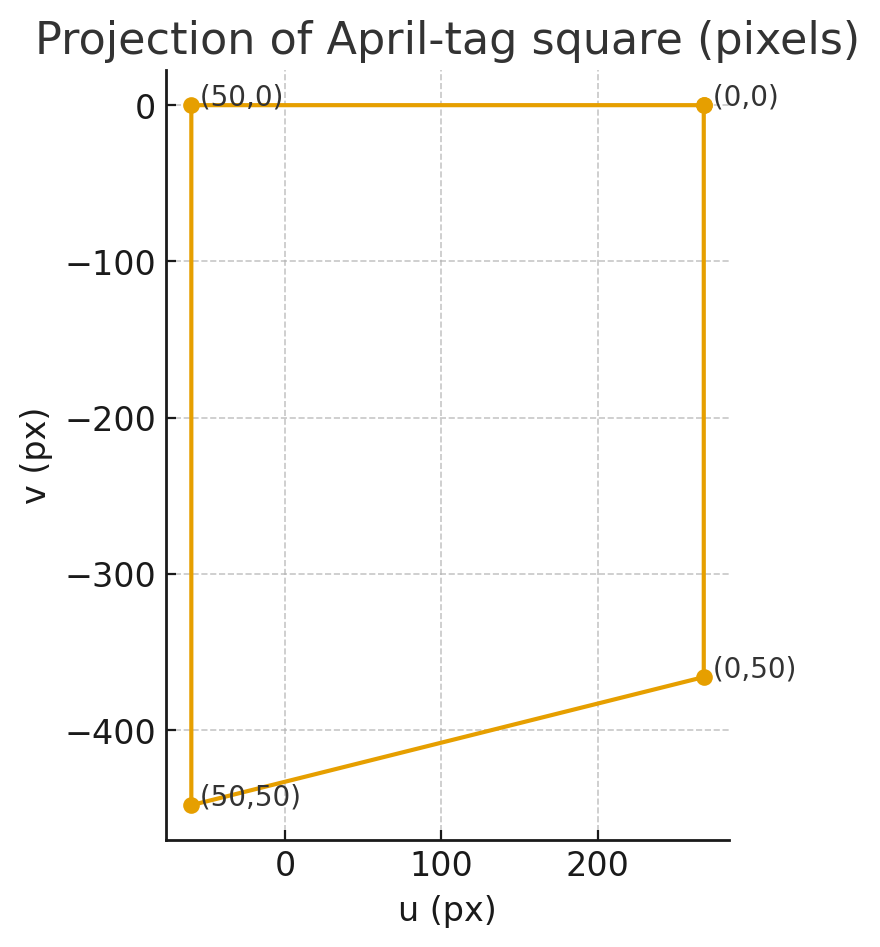
\includegraphics[width=0.6\textwidth]{./media/tag_quadrilateral.png}
    \caption{Projected April Tag Corners in Image Plane}
    \label{fig:tag_projection}
\end{figure}

\subsection*{4.7}

For a tag-plane point \((X_A,Y_A,0)\) the (unnormalized) homogeneous image point is
\[
\tilde{\mathbf{x}}
~\sim~
\begin{bmatrix}
f\big(c\,(X_A-d_{xA}) + s\,d_{zA}\big)\\[2pt]
f\,(Y_A-h)\\[2pt]
s\,(X_A-d_{xA}) - c\,d_{zA}
\end{bmatrix},
\qquad c=\cos 30^\circ,\; s=\sin 30^\circ .
\]
Hence, for the square \((0,0),(a,0),(a,a),(0,a)\),
\[
\boxed{
\begin{aligned}
\tilde{\mathbf{x}}_{00} &~\sim~
\begin{bmatrix}
f(-c\,d_{xA}+s\,d_{zA})\\[2pt]
f(-h)\\[2pt]
-\,s\,d_{xA}-c\,d_{zA}
\end{bmatrix},&
\tilde{\mathbf{x}}_{a0} &~\sim~
\begin{bmatrix}
f\big(c(a-d_{xA})+s\,d_{zA}\big)\\[2pt]
f(-h)\\[2pt]
s(a-d_{xA})-c\,d_{zA}
\end{bmatrix},\\[10pt]
\tilde{\mathbf{x}}_{aa} &~\sim~
\begin{bmatrix}
f\big(c(a-d_{xA})+s\,d_{zA}\big)\\[2pt]
f(a-h)\\[2pt]
s(a-d_{xA})-c\,d_{zA}
\end{bmatrix},&
\tilde{\mathbf{x}}_{0a} &~\sim~
\begin{bmatrix}
f(-c\,d_{xA}+s\,d_{zA})\\[2pt]
f(a-h)\\[2pt]
-\,s\,d_{xA}-c\,d_{zA}
\end{bmatrix}.
\end{aligned}
}
\]
(If you prefer normalized coordinates, divide each vector by its third component to get \((u,v,1)^\top\).)

\subsection*{4.8}
Let the four (unnormalized) homogeneous image points from Q4.7 be
\[
\tilde{\mathbf{x}}(X_A,Y_A)\sim
\begin{bmatrix}
f\big(c\,(X_A-d_{xA})+s\,d_{zA}\big)\\[2pt]
f\,(Y_A-h)\\[2pt]
s\,(X_A-d_{xA})-c\,d_{zA}
\end{bmatrix},
\qquad c=\cos30^\circ,\; s=\sin30^\circ .
\]
The homogeneous line through two points is \(\ell=\tilde{\mathbf{x}}_1\times\tilde{\mathbf{x}}_2\).
Using the four square corners \((0,0),(a,0),(a,a),(0,a)\) and simplifying
(\(c^2+s^2=1\)), we obtain the four side lines
(up to a nonzero scale):

\[
\boxed{
\begin{aligned}
\text{Bottom }(Y_A=0):\quad
&\ell_b=(A_b,B_b,C_b)=\big(\,-h\,s,\ \ -d_{zA},\ \ c\,f\,h\big),\\[4pt]
\text{Top }(Y_A=a):\quad
&\ell_t=(A_t,B_t,C_t)=\big(\ s\,(h-a),\ \ d_{zA},\ \ c\,f\,(a-h)\big),\\[4pt]
\text{Right }(X_A=a):\quad
&\ell_r=(A_r,B_r,C_r)=\big(\ c\,d_{zA}-s\,(a-d_{xA}),\ \ 0,\ \ f\big(c\,(a-d_{xA})+s\,d_{zA}\big)\big),\\[4pt]
\text{Left }(X_A=0):\quad
&\ell_\ell=(A_\ell,B_\ell,C_\ell)=\big(\ -(c\,d_{zA}+s\,d_{xA}),\ \ 0,\ \ f\big(c\,d_{xA}-s\,d_{zA}\big)\big).
\end{aligned}}
\]

Each side satisfies \(A\,u + B\,v + C\,w = 0\) (with \((u,v,w)^\top\) the homogeneous image
coordinates). Any nonzero scalar multiple of a line triple represents the same line.

\subsection*{4.9}
\paragraph{Q4.9 — Vanishing points from the two pairs of sides}

On the April–tag plane \(Z_A=0\), the image mapping is the homography
\[
H \;=\; K\,[\,r_1\;\; r_2\;\; T\,],\qquad
r_1=\begin{bmatrix}c\\0\\s\end{bmatrix},\;
r_2=\begin{bmatrix}0\\1\\0\end{bmatrix},
\]
with \(c=\cos 30^\circ,\; s=\sin 30^\circ\) and \(K=\mathrm{diag}(f,f,1)\).
A vanishing point for directions parallel to a plane direction \(\mathbf{d}\) is
\(\; \tilde{\mathbf{v}} \sim K\,R\,\mathbf{d}\), so for the two orthogonal directions:

\[
\boxed{
\tilde{\mathbf{v}}_X \;\sim\; K\,r_1
= \begin{bmatrix} f c \\[2pt] 0 \\[2pt] s \end{bmatrix},
\qquad
\tilde{\mathbf{v}}_Y \;\sim\; K\,r_2
= \begin{bmatrix} 0 \\[2pt] f \\[2pt] 0 \end{bmatrix}.
}
\]

Interpretation:
- \(\tilde{\mathbf{v}}_X\) is the vanishing point for the pair of sides parallel to the \(X_A\)-axis
  (the “top” and “bottom” edges of the square). In Euclidean image coordinates,
  \((u,v) = \big(\tfrac{f c}{s},\,0\big) = (\sqrt{3}\,f,\,0)\).
- \(\tilde{\mathbf{v}}_Y\) is the vanishing point for the pair of sides parallel to the \(Y_A\)-axis
  (the “left” and “right” edges). Since \(w=0\), it lies at infinity in the vertical
  image direction, consistent with these two sides projecting as parallel vertical lines.


\subsection*{4.10}
\paragraph{Q4.10 — Horizon (vanishing line) of the April–tag plane}
For the tag plane \(Z_A=0\), the horizon (image of the line at infinity of the plane)
is
\[
\ell_\infty^\text{tag} \;\sim\; K^{-\top} R\,\mathbf{n},\qquad
\mathbf{n}=\begin{bmatrix}0\\0\\1\end{bmatrix}.
\]
With \(R=R_y(-\theta)\) (\(\theta=30^\circ\)), \(c=\cos\theta\), \(s=\sin\theta\),
the third column of \(R\) is \(r_3=[-s,\,0,\,c]^\top\). For
\(K=\mathrm{diag}(f,f,1)\),
\[
\boxed{\;
\ell_\infty^\text{tag} \;\sim\; K^{-\top} r_3
= \begin{bmatrix} -\,s/f \\[2pt] 0 \\[2pt] c \end{bmatrix}
\;\equiv\; \begin{bmatrix} -\,s \\[2pt] 0 \\[2pt] f\,c \end{bmatrix}.
\;}
\]
Thus the line equation \(A\,u + B\,v + C\,w=0\) is
\[
(-s)\,u + 0\cdot v + (f c)\,w = 0.
\]
In Euclidean pixel coordinates \((w=1)\),
\[
\boxed{\; u \;=\; \dfrac{f c}{s} \;=\; \sqrt{3}\,f \quad(\theta=30^\circ). \;}
\]
(Any nonzero scalar multiple of \(\ell_\infty^\text{tag}\) represents the same line.)

\subsection*{4.11}
\paragraph{Q4.11 — Coordinates of point \(P\) on the wall (tag plane)}
Let \(P\) have pixel coordinates \((u_P,v_P)\) in the image. The April–tag lies in the plane \(Z_A=0\),
and the plane-to-image homography from Q4.4 is
\[
H \;=\; K\,[\,r_1\;\; r_2\;\; T\,],\qquad
r_1=\begin{bmatrix}c\\0\\s\end{bmatrix},\;
r_2=\begin{bmatrix}0\\1\\0\end{bmatrix},\;
T=\begin{bmatrix}-c\,d_{xA}+s\,d_{zA}\\ -h\\ -s\,d_{xA}-c\,d_{zA}\end{bmatrix},
\]
with \(K=\mathrm{diag}(f,f,1)\), \(c=\cos 30^\circ\), \(s=\sin 30^\circ\).
The wall (tag) coordinates \((X_A,Y_A,1)^\top\) of \(P\) are obtained by back–projecting via
\[
\begin{bmatrix}X_A\\[2pt] Y_A\\[2pt] 1\end{bmatrix}
~\sim~
H^{-1}\begin{bmatrix}u_P\\[2pt] v_P\\[2pt] 1\end{bmatrix}.
\]

\medskip
\textbf{Closed form (solving the projection equations).}
For any image point \((u,v)\) that comes from \((X_A,Y_A,0)\), we derived in Q4.3:
\[
u \;=\; f\,\frac{c\,(X_A-d_{xA}) + s\,d_{zA}}{\,D\,},\qquad
v \;=\; f\,\frac{Y_A - h}{\,D\,},\qquad
D \;=\; s\,(X_A-d_{xA}) - c\,d_{zA}.
\]
Solving for \((X_A,Y_A)\) in terms of \((u,v)\) gives
\[
\boxed{\;
X_A \;=\; d_{xA} \;+\; d_{zA}\,\frac{\ \dfrac{u\,c}{f} + s\ }{\ \dfrac{u\,s}{f} - c\ },\qquad
Y_A \;=\; h \;+\; \frac{v}{f}\,d_{zA}\!\left(\, s\,\frac{\ \dfrac{u\,c}{f} + s\ }{\ \dfrac{u\,s}{f} - c\ } - c \right).
\;}
\]
Thus, for \(P=(u_P,v_P)\), substitute \(u\!=\!u_P\), \(v\!=\!v_P\) in the boxed formulas to obtain \((X_A,Y_A)\).

\medskip
\textit{Numeric template (if needed):} with \(f=1000\), \(h=0\), \(d_{xA}=d_{zA}=100\),
\(c=\sqrt{3}/2\), \(s=1/2\), plug these constants into the same expressions to evaluate \((X_A,Y_A)\) for your measured \((u_P,v_P)\).

\subsection*{Bonus 1}

\paragraph{Setup.} Since the world Z-axis aligns with gravity and the robot knows gravity in camera coordinates, the rotation between world and camera is a pure yaw about the Z-axis:
\[
R = R_z(\theta) = \begin{bmatrix}
\cos\theta & -\sin\theta & 0 \\
\sin\theta & \cos\theta & 0 \\
0 & 0 & 1
\end{bmatrix}
\]

The camera projection equations are:
\[
\lambda_i \begin{bmatrix} x_i \\ y_i \\ 1 \end{bmatrix} = R \begin{bmatrix} X_i \\ Y_i \\ Z_i \end{bmatrix} + \mathbf{t}
\]

where $\mathbf{t} = [t_x, t_y, t_z]^T$ and $i = 1, 2$.

\paragraph{Step 1: Write the projection equations.}
For each point $i$:
\begin{align}
\lambda_i x_i &= \cos\theta \cdot X_i - \sin\theta \cdot Y_i + t_x \\
\lambda_i y_i &= \sin\theta \cdot X_i + \cos\theta \cdot Y_i + t_y \\
\lambda_i &= Z_i + t_z
\end{align}

\paragraph{Step 2: Eliminate translation parameters.}
From equations (3): $\lambda_1 = Z_1 + t_z$ and $\lambda_2 = Z_2 + t_z$

Therefore: $t_z = \lambda_1 - Z_1 = \lambda_2 - Z_2$

This gives us: $\lambda_1 - \lambda_2 = Z_1 - Z_2$

From equations (1) and (2), we can eliminate $t_x$ and $t_y$:
\begin{align}
\lambda_1 x_1 - \lambda_2 x_2 &= \cos\theta(X_1 - X_2) - \sin\theta(Y_1 - Y_2) \\
\lambda_1 y_1 - \lambda_2 y_2 &= \sin\theta(X_1 - X_2) + \cos\theta(Y_1 - Y_2)
\end{align}

\paragraph{Step 3: Express in terms of one unknown.}
Let $\lambda = \lambda_1$. Then $\lambda_2 = \lambda - (Z_1 - Z_2)$.

Substituting into equations (4) and (5):
\begin{align}
\lambda x_1 - (\lambda - (Z_1 - Z_2))x_2 &= \cos\theta(X_1 - X_2) - \sin\theta(Y_1 - Y_2) \\
\lambda y_1 - (\lambda - (Z_1 - Z_2))y_2 &= \sin\theta(X_1 - X_2) + \cos\theta(Y_1 - Y_2)
\end{align}

Simplifying:
\begin{align}
\lambda(x_1 - x_2) + (Z_1 - Z_2)x_2 &= \cos\theta(X_1 - X_2) - \sin\theta(Y_1 - Y_2) \\
\lambda(y_1 - y_2) + (Z_1 - Z_2)y_2 &= \sin\theta(X_1 - X_2) + \cos\theta(Y_1 - Y_2)
\end{align}

\paragraph{Step 4: Solve for $\cos\theta$ and $\sin\theta$.}
Let:
\begin{align}
A &= \lambda(x_1 - x_2) + (Z_1 - Z_2)x_2 \\
B &= \lambda(y_1 - y_2) + (Z_1 - Z_2)y_2 \\
C &= X_1 - X_2 \\
D &= Y_1 - Y_2
\end{align}

Then we have the system:
\begin{align}
A &= C\cos\theta - D\sin\theta \\
B &= C\sin\theta + D\cos\theta
\end{align}

Solving for $\cos\theta$ and $\sin\theta$:
\begin{align}
\cos\theta &= \frac{AC + BD}{C^2 + D^2} \\
\sin\theta &= \frac{BC - AD}{C^2 + D^2}
\end{align}

\paragraph{Step 5: Polynomial constraint.}
Using $\cos^2\theta + \sin^2\theta = 1$:
\[
\left(\frac{AC + BD}{C^2 + D^2}\right)^2 + \left(\frac{BC - AD}{C^2 + D^2}\right)^2 = 1
\]

This simplifies to:
\[
(AC + BD)^2 + (BC - AD)^2 = (C^2 + D^2)^2
\]

Expanding and substituting the expressions for $A$ and $B$ in terms of $\lambda$:
\[
\boxed{
\left[\lambda(x_1-x_2) + (Z_1-Z_2)x_2\right]^2 + \left[\lambda(y_1-y_2) + (Z_1-Z_2)y_2\right]^2 = (X_1-X_2)^2 + (Y_1-Y_2)^2
}
\]

This is a quadratic equation in $\lambda$.

\paragraph{Step 6: Complete solution.}
1. Solve the quadratic equation for $\lambda = \lambda_1$
2. Compute $\lambda_2 = \lambda_1 - (Z_1 - Z_2)$
3. Calculate $\cos\theta$ and $\sin\theta$ using equations (15) and (16)
4. Find $\theta = \arctan2(\sin\theta, \cos\theta)$
5. Recover translations:
   \begin{align}
   t_x &= \lambda_1 x_1 - \cos\theta \cdot X_1 + \sin\theta \cdot Y_1 \\
   t_y &= \lambda_1 y_1 - \sin\theta \cdot X_1 - \cos\theta \cdot Y_1 \\
   t_z &= \lambda_1 - Z_1
   \end{align}

\textbf{Final Answer:} The unknowns $(\theta, t_x, t_y, t_z)$ are determined by solving the quadratic constraint equation and applying the recovery formulas above.


gggg

\section*{Bonus (15 pts): P2P with Gravity — Solve for \(\theta,t_x,t_y,t_z\)}

\paragraph{Setup.}
Camera is calibrated, so image points are in normalized (calibrated) coordinates
\(\mathbf{d}_i=[x_i,y_i,1]^\top\).
World \(Z\)-axis is gravity; the camera knows gravity in its own frame, so the
rotation from world to camera is a known roll–pitch \(R_g\) composed with an
unknown yaw \(\theta\) about the (known) world \(Z\)-axis:
\[
R(\theta)=R_z(\theta)\,R_g,\qquad
R_z(\theta)=
\begin{bmatrix}
\cos\theta&-\sin\theta&0\\
\sin\theta& \cos\theta&0\\
0&0&1
\end{bmatrix}.
\]
Two 3D–2D correspondences \((X_i,Y_i,Z_i)\leftrightarrow (x_i,y_i)\), \(i=1,2\), obey
\[
s_i\,\mathbf{d}_i \;=\; R(\theta)\,\mathbf{P}_i + \mathbf{t},
\qquad \mathbf{P}_i=\begin{bmatrix}X_i\\Y_i\\Z_i\end{bmatrix},\;
\mathbf{t}=\begin{bmatrix}t_x\\t_y\\t_z\end{bmatrix}.
\]

\paragraph{Eliminate translation (and scales).}
Subtract the two projection equations:
\[
s_1\,\mathbf{d}_1 - s_2\,\mathbf{d}_2 \;=\; R(\theta)\,\Delta\mathbf{P},
\qquad \Delta\mathbf{P}=\mathbf{P}_1-\mathbf{P}_2.
\]
Take the cross product with \(\mathbf{d}_1\) and \(\mathbf{d}_2\) to eliminate the scales:
\[
\mathbf{d}_1 \times \big(R(\theta)\,\Delta\mathbf{P}\big) \;=\; -\,s_2\,(\mathbf{d}_1\times\mathbf{d}_2),\qquad
\mathbf{d}_2 \times \big(R(\theta)\,\Delta\mathbf{P}\big) \;=\;\;\; s_1\,(\mathbf{d}_1\times\mathbf{d}_2).
\]
Hence both vectors on the left are \emph{collinear} with \(\mathbf{k}:=\mathbf{d}_1\times\mathbf{d}_2\).
This yields two scalar parallelism constraints.

\paragraph{Reduce to a single unknown \(\theta\).}
Define the known vector
\[
\mathbf{u}:=R_g\,\Delta\mathbf{P} \quad\Rightarrow\quad
R(\theta)\,\Delta\mathbf{P}
=R_z(\theta)\,\mathbf{u}
=\begin{bmatrix}
c\,u_x - s\,u_y\\
s\,u_x + c\,u_y\\
u_z
\end{bmatrix},\quad c=\cos\theta,\ s=\sin\theta.
\]
With \(\mathbf{d}_i=[x_i,y_i,1]^\top\), compute
\[
\mathbf{q}_i(\theta):=\mathbf{d}_i\times\big(R_z(\theta)\mathbf{u}\big)
=
\begin{bmatrix}
y_i\,u_z - (s\,u_x + c\,u_y)\\[2pt]
(c\,u_x - s\,u_y) - x_i\,u_z\\[2pt]
x_i(s\,u_x + c\,u_y) - y_i(c\,u_x - s\,u_y)
\end{bmatrix}.
\]
Parallelism \(\mathbf{q}_i(\theta)\parallel \mathbf{k}\) is equivalent to
\((\mathbf{q}_i)_x\,k_y - (\mathbf{q}_i)_y\,k_x=0\), where
\(\mathbf{k}=\mathbf{d}_1\times\mathbf{d}_2=[\,y_1-y_2,\; x_2-x_1,\; x_1y_2-y_1x_2\,]^\top\).
For \(i=1\) and \(i=2\) this gives two \emph{linear} equations in \(c,s\):
\[
\alpha_i\,c \;+\; \beta_i\,s \;+\; \gamma_i \;=\; 0,\qquad i=1,2,
\]
with known coefficients
\[
\begin{aligned}
\alpha_i &= (x_2-x_1)\,u_x \;+\; (y_1-y_2)\,u_y,\\
\beta_i  &= -\,(x_2-x_1)\,u_y \;+\; (y_1-y_2)\,u_x,\\
\gamma_i &= -\,u_z\big((y_i)(x_2-x_1) + (x_i)(y_1-y_2)\big).
\end{aligned}
\]
(These arise by expanding \((\mathbf{q}_i)_x\,k_y - (\mathbf{q}_i)_y\,k_x=0\).)

Stack them:
\[
\begin{bmatrix}\alpha_1 & \beta_1\\ \alpha_2 & \beta_2\end{bmatrix}
\begin{bmatrix}c\\s\end{bmatrix}
= -\begin{bmatrix}\gamma_1\\\gamma_2\end{bmatrix}.
\]
Solve formally for \(c,s\) as functions of a common scale, then enforce \(c^2+s^2=1\).
Equivalently, substitute \(c=\tfrac{1-t^2}{1+t^2},\ s=\tfrac{2t}{1+t^2}\) with \(t=\tan(\theta/2)\).
Each linear equation becomes a rational equation in \(t\); clearing denominators yields a
\emph{quadratic} in \(t\). Intersecting the two gives a single quadratic (they are consistent),
whose real roots are the candidates for \(\theta\). Pick the root that yields positive
depths (see below).

\paragraph{Recover translation and scales.}
With \(\theta\) known, obtain \(s_1,s_2\) from the collinearity relations:
\[
s_2 \;=\; -\,\frac{\big(\mathbf{d}_1\times (R(\theta)\Delta\mathbf{P})\big)\cdot \mathbf{k}}
{\ \mathbf{k}\cdot\mathbf{k}\ },\qquad
s_1 \;=\;\;\frac{\big(\mathbf{d}_2\times (R(\theta)\Delta\mathbf{P})\big)\cdot \mathbf{k}}
{\ \mathbf{k}\cdot\mathbf{k}\ }.
\]
Then recover translation from either correspondence:
\[
\boxed{\ \mathbf{t}
= s_1\,\mathbf{d}_1 - R(\theta)\,\mathbf{P}_1
= s_2\,\mathbf{d}_2 - R(\theta)\,\mathbf{P}_2\ }.
\]
(Using both gives a consistency check; numerical implementation can average them.)

\paragraph{Summary (algorithmic form).}
\begin{enumerate}
\item Compute \(\mathbf{u}=R_g\,(\mathbf{P}_1-\mathbf{P}_2)\) and \(\mathbf{k}=\mathbf{d}_1\times\mathbf{d}_2\).
\item Form two linear equations \(\alpha_i c+\beta_i s+\gamma_i=0\) (\(i=1,2\)) from parallelism.
\item Substitute \(c=\tfrac{1-t^2}{1+t^2},\ s=\tfrac{2t}{1+t^2}\) to get a quadratic in \(t=\tan(\theta/2)\).
\item Choose the root that yields positive depths; set \(\theta=2\arctan t\).
\item Compute \(s_1,s_2\) from the cross-product formulas; then \(\mathbf{t}\) from one correspondence.
\end{enumerate}
This solves \((\theta,t_x,t_y,t_z)\) from two 3D--2D points when roll and pitch are known from gravity.


\paragraph{Bonus 2 — Why gravity + two points suffice; singular cases}

\textbf{Why it is sufficient (qualitative).}
Knowing gravity in the camera frame aligns the camera’s vertical with the world’s
\(Z\)-axis, so roll and pitch are fixed. The only rotational DoF left is the yaw \(\theta\)
about the (known) world \(Z\)-axis. The remaining unknowns are thus
\(\{\theta,t_x,t_y,t_z\}\) (four scalars).
With a calibrated camera, each 3D--2D correspondence \((X_i,Y_i,Z_i)\leftrightarrow(x_i,y_i)\)
provides two independent scalar equations. Two correspondences yield four equations,
which is exactly enough to solve for the four unknowns. Operationally, one can
eliminate translation by subtracting the two projection equations, solve for \(\theta\),
then back-substitute to recover \((t_x,t_y,t_z)\).

\textbf{Singular (unobservable) configurations.}
\begin{itemize}
  \item \emph{Vertical-only 3D baseline:} If the two world points differ only along gravity,
  \(\Delta\mathbf{P}\parallel \mathbf{e}_Z\), then yaw about \(Z\) does not affect their relative
  projection; \(\theta\) becomes unobservable.
  \item \emph{Coincident/parallel image rays:} If the calibrated image directions satisfy
  \(\mathbf{d}_1=\mathbf{d}_2\) (coincident image points or parallel rays),
  then \(\mathbf{d}_1\times \mathbf{d}_2=\mathbf{0}\) and the elimination constraint degenerates.
  \item \emph{Trivial 3D baseline:} If the two 3D points coincide (\(\Delta\mathbf{P}=\mathbf{0}\)),
  there is no geometric constraint to recover pose.
\end{itemize}
(Configurations that are nearly vertical or nearly parallel are numerically ill-conditioned,
even if not strictly singular.)

\end{document}
